% nff — power budget for a BLE-only, battery-powered ESP32 sensor node
%
% Build:  pdflatex ble-power-budget.tex   (run twice for the ToC / references)
% Deps:   circuitikz, booktabs, siunitx, xcolor, geometry, fancyhdr, enumitem
%         Same set as datasheet.tex — a standard TeX Live / MiKTeX "full" install.

\documentclass[11pt,a4paper]{article}

\usepackage[margin=22mm]{geometry}
\usepackage{booktabs}
\usepackage{siunitx}
\usepackage{circuitikz}
\usetikzlibrary{decorations.pathreplacing}
\usepackage{xcolor}
\usepackage{fancyhdr}
\usepackage{enumitem}
\usepackage{amsmath}
\usepackage{tabularx}
\usepackage[hidelinks]{hyperref}

\sisetup{
  per-mode              = symbol,
  range-units           = single,
  detect-weight         = true,
  group-minimum-digits  = 4,
}
% dBm is not an siunitx built-in. Bytes and calendar units (\day/\month/\year clash with
% TeX primitives) are deliberately written as plain text throughout.
\DeclareSIUnit{\dBm}{dBm}

\definecolor{warn}{RGB}{176,0,32}
\definecolor{ok}{RGB}{0,120,60}
\providecommand{\good}[1]{\textcolor{ok}{\textbf{#1}}}
\providecommand{\bad}[1]{\textcolor{warn}{\textbf{#1}}}
\newcommand{\yes}{\textcolor{ok}{\textbf{yes}}}
\newcommand{\no}{\textcolor{warn}{\textbf{no}}}
\newcommand{\pass}{\textcolor{ok}{\textbf{PASS}}}
\newcommand{\fail}{\textcolor{warn}{\textbf{FAIL}}}
\newcommand{\meas}{\textcolor{ok}{$^{\ast}$}}
\newcommand{\mock}{\textcolor{warn}{$\dagger$}}

\pagestyle{fancy}
\fancyhf{}
\lhead{\small nff --- BLE power budget}
\chead{\small \textcolor{warn}{\textbf{MOCK VALUES}}}
\rhead{\small Rev.\ A --- 2026-07-13}
\cfoot{\small \thepage}

\title{\textbf{nff on battery}\\[2mm]
\large Energy cost of the nff toolchain on ESP32, and the parameter set for a\\
BLE-only \SI{6000}{\milli\ampere\hour} / 12-month sensor node\\[1mm]
\normalsize Power budget --- Revision A}
\author{Target: ESP32-WROOM-32E, BLE-only, one gateway per site}
\date{2026-07-13}

\begin{document}
\maketitle
\thispagestyle{fancy}

\noindent
\fcolorbox{warn}{white}{\parbox{0.97\textwidth}{%
\textbf{\mock\ Every current, duration and energy figure in this document is a placeholder.}
None has been measured. They are internally consistent and drawn from the ESP32 datasheet's order
of magnitude, and they are good enough to decide \emph{feasibility} --- which is what
\S\ref{sec:verdict} does --- but they are not good enough to sign a contract against. The rig that
will replace them is specified in \texttt{datasheet.tex}, and \S\ref{sec:lie} explains why that
rig \textbf{cannot measure the most important number in this document} (the sleep floor), and what
instrument can.}}

\begin{abstract}
\noindent
This document does three things. It gives the energy cost of every \texttt{nff} operation that
runs on an ESP32 (\S\ref{sec:tools}, mock values). It gives the \texttt{nff} SDK settings that
matter under a power constraint, and states plainly the two things the SDK cannot currently do at
all (\S\ref{sec:sdk}). And it gives the ESP32/BLE parameter set for the stated duty cycle
(\S\ref{sec:params}--\S\ref{sec:adv}).

\medskip
\noindent
\textbf{The headline is a distinction, not a number.} The requirement says the device ``wakes for
approximately \SI{30}{\second} every \SI{5}{\minute}''. \emph{Awake for \SI{30}{\second}} and
\emph{the CPU runs for \SI{30}{\second}} are not the same requirement, and the feasibility of this
product turns entirely on which one gets built. The literal reading --- wake, advertise in a busy
loop for \SI{30}{\second}, sleep --- yields \textbf{6 weeks} on a \SI{6000}{\milli\ampere\hour}
cell, and \textbf{20 days} if it is built on a devkit board. The target is 12 months. That gap is
not closable by tuning the radio, because the radio is not where the energy goes.

\medskip
\noindent
Two designs do close, with roughly \num{1.5}$\times$ margin, and both are given in full
(\S\ref{sec:verdict}). One shortens the CPU-active window to \SI{2.5}{\second}. The other keeps
the literal \SI{30}{\second} window but spends \SI{29}{\second} of it in automatic light sleep,
with the BT controller holding the advertising timing. They land within \SI{5}{\percent} of each
other --- which is itself the most useful result here: once the CPU is asleep, the \textbf{boot
sequence, not the radio and not the wake duration, becomes the largest single line item in the
budget.}
\end{abstract}

\clearpage
\tableofcontents
\clearpage

% ---------------------------------------------------------------------------
\section{Verdict}
\label{sec:verdict}

\subsection{The budget}

\begin{center}
\begin{tabularx}{\textwidth}{lXl}
\toprule
\textbf{Quantity} & \textbf{Derivation} & \textbf{Value} \\
\midrule
Battery, nominal        & Given & \SI{6000}{\milli\ampere\hour} \\
Battery, \emph{usable}  & \SI{85}{\percent} derate: self-discharge, low-temperature capacity loss, cut-off voltage headroom (\S\ref{sec:battery}) & \SI{5100}{\milli\ampere\hour} \\
Target life             & Given: 12 months & \SI{8760}{\hour} \\
\midrule
\textbf{Mean current budget} & $\SI{5100}{\milli\ampere\hour} / \SI{8760}{\hour}$ & \textbf{\SI{582}{\micro\ampere}} \\
Cycles per year         & $\SI{8760}{\hour}\times\SI{3600}{\second\per\hour} / \SI{300}{\second}$ & \num{105120} \\
\textbf{Charge budget per cycle} & $\SI{582}{\micro\ampere}\times\SI{300}{\second}$ & \textbf{\SI{48.5}{\micro\ampere\hour}} \\
\bottomrule
\end{tabularx}
\end{center}

\noindent
Everything the device does in a \SI{5}{\minute} cycle --- boot, initialise the BT controller, read
the sensor, advertise, tear down, and sleep for the remaining \SI{4.5}{\minute} --- must fit inside
\SI{48.5}{\micro\ampere\hour}. That is the whole problem, stated once.

\subsection{Four designs}

\begin{center}
\begin{tabularx}{\textwidth}{lllllX}
\toprule
& \textbf{Board} & \textbf{CPU-active} & \textbf{Sleep floor} & \textbf{$I_\text{mean}$} & \textbf{Life} \\
\midrule
\textbf{D0} & Devkit & \SI{31.2}{\second} & \SI{6.5}{\milli\ampere} & \SI{10.8}{\milli\ampere} & \textcolor{warn}{\textbf{20 days}} \\
\textbf{D1} & Custom & \SI{31.2}{\second} & \SI{20}{\micro\ampere}  & \SI{5.01}{\milli\ampere} & \textcolor{warn}{\textbf{6.1 weeks}} \\
\textbf{D2} & Custom & \SI{2.5}{\second}  & \SI{20}{\micro\ampere}  & \SI{380}{\micro\ampere}  & \textcolor{ok}{\textbf{18.4 months}} \\
\textbf{D3} & Custom & \SI{1.2}{\second}  & \SI{20}{\micro\ampere}  & \SI{394}{\micro\ampere}  & \textcolor{ok}{\textbf{17.7 months}} \\
\midrule
\multicolumn{4}{l}{\textit{Budget --- mean current must not exceed}} & \textbf{\SI{582}{\micro\ampere}} & \textit{12 months} \\
\bottomrule
\end{tabularx}
\end{center}

\noindent
D3's \SI{1.2}{\second} of CPU-active time sits inside a \SI{30}{\second} advertising window; the
CPU is in light sleep for the other \SI{29}{\second} (\S1.6).

\begin{description}[style=nextline,leftmargin=6mm]
  \item[D0 --- the literal spec, built the obvious way, on a devkit.] \fail\ by \num{18}$\times$.
        Note that D0 fails \emph{on its sleep floor alone}: \SI{6.5}{\milli\ampere} of AMS1117
        quiescent current, CP2102 bridge and power LED, drawn for \SI{4.5}{\minute} of every
        cycle, is already \num{11}$\times$ the entire budget before the firmware executes one
        instruction (\S\ref{sec:sleep}).
  \item[D1 --- the literal spec, on a proper board.] \fail\ by \num{8.6}$\times$. The board is
        fixed; the firmware is not. \SI{30}{\second} of CPU-active time at roughly
        \SI{48}{\milli\ampere} is \SI{400}{\micro\ampere\hour} per cycle against a
        \SI{48.5}{\micro\ampere\hour} budget.
  \item[D2 --- short window. \emph{Recommended.}] \pass, margin \num{1.53}$\times$. Identical
        behaviour from the gateway's point of view; the wake window is \SI{2.5}{\second} instead
        of \SI{30}{\second}. No extra parts.
  \item[D3 --- literal \SI{30}{\second} window, held in light sleep.] \pass, margin
        \num{1.48}$\times$. Preserves the stated \SI{30}{\second} advertising window verbatim; the
        CPU only \emph{runs} for \SI{1.2}{\second} of it. Costs a \SI{32.768}{\kilo\hertz} crystal
        on the BOM.
\end{description}

\subsection{The closure equation}

For a period $T$, a sleep floor $I_\text{sleep}$ and a mean CPU-active current $I_\text{awake}$,
the longest CPU-active window that still meets a mean-current budget $I_\text{budget}$ is
\[
\boxed{\;
t_\text{on,max} \;=\; T \cdot \frac{I_\text{budget} - I_\text{sleep}}{I_\text{awake} - I_\text{sleep}}
\;}
\qquad\Longrightarrow\qquad
\SI{300}{\second}\cdot\frac{\SI{582}{\micro\ampere} - \SI{20}{\micro\ampere}}
                           {\SI{43.2}{\milli\ampere} - \SI{20}{\micro\ampere}}
\;=\; \SI{3.9}{\second}.
\]

\noindent
\textbf{\SI{3.9}{\second} is the hard ceiling on CPU-active time per \SI{5}{\minute} cycle.} Every
design decision in this document is downstream of that one number. Spending the entire
\SI{6000}{\milli\ampere\hour} with no derate at all buys \SI{4.6}{\second} --- so the ceiling is
robust: it does not hinge on how generous the battery derating is.

\medskip
\noindent
\fcolorbox{warn}{white}{\parbox{0.97\textwidth}{%
\textbf{Note what the equation is \emph{insensitive} to.} Halving $I_\text{awake}$ from
\SI{43}{\milli\ampere} to \SI{21}{\milli\ampere} --- an aggressive, expensive, silicon-level win
--- only doubles $t_\text{on,max}$, to \SI{7.8}{\second}. That is still nowhere near
\SI{30}{\second}. \textbf{No achievable reduction in current closes a \SI{30}{\second} CPU-active
window.} Only reducing the \emph{time} does. This is why the recommendation is a
firmware-architecture change and not a component selection.}}

\subsection{Why the verdict survives the mock values}
\label{sec:robust}

\noindent
Every current in this document is invented (\S\ref{sec:lie}, L1), which invites the obvious
objection: \emph{if the inputs are made up, why believe the conclusion?} Because the conclusion
does not use them. The failure of D1 can be shown with no number from this document at all.

\medskip
\noindent
Grant the design every advantage:

\begin{itemize}[leftmargin=*,nosep]
  \item \textbf{No battery derate.} Spend the entire \SI{6000}{\milli\ampere\hour}, not the
        \SI{5100}{\milli\ampere\hour} of \S1.1. Budget becomes \SI{685}{\micro\ampere}.
  \item \textbf{A free sleep.} Set $I_\text{sleep} = 0$. The device costs nothing for
        \SI{4.5}{\minute} of every cycle.
  \item \textbf{A silent radio.} No advertising, no TX. The CPU merely \emph{runs}.
\end{itemize}

\medskip
\noindent
The duty cycle is fixed by the requirement at $\SI{30}{\second}/\SI{300}{\second} =
\SI{10}{\percent}$. So the maximum current the device may draw while awake is
\[
I_\text{awake,max} \;=\; \frac{\SI{685}{\micro\ampere}}{0.10} \;=\; \SI{6.85}{\milli\ampere}.
\]

\noindent
\fcolorbox{warn}{white}{\parbox{0.97\textwidth}{%
\textbf{There is no operating mode in which an ESP32 executes code at \SI{6.85}{\milli\ampere}.}
Espressif's datasheet puts the \emph{lowest} CPU-executing state --- modem sleep, \SI{80}{\mega\hertz},
radio off --- at roughly \SIrange{20}{31}{\milli\ampere}. The requirement is therefore over budget
by at least \num{3}$\times$ \textbf{with a perfect battery, a free sleep, and the radio switched
off}, before the sensor is read or a single advertisement is sent.

\medskip
The mock values decide whether the answer is ``6 weeks'' or ``9 weeks''. \textbf{They do not decide
whether it fails.} That conclusion rests on three numbers, none of them ours: the customer's
\SI{6000}{\milli\ampere\hour}, the customer's \SI{10}{\percent} duty cycle, and Espressif's
datasheet.}}

\medskip
\noindent
\textbf{What the mock values \emph{do} decide is the margin on D2 and D3} --- whether they land at
18 months, or at 11, or at 30. Those figures are not yet trustworthy, and \S\ref{sec:measure}
gives the single measurement that makes them so.

\subsection{The one measurement that converts this document --- \good{TAKEN 2026-07-14}}
\label{sec:measure}

\noindent
The verdict hinges on exactly one quantity: $I_\text{awake}$, the mean current with the CPU
running and BLE advertising. Everything else is either arithmetic or a design target.

\medskip
\noindent
\noindent
\fcolorbox{ok}{white}{\parbox{\dimexpr\textwidth-2\fboxsep-2\fboxrule}{%
\textbf{Done --- for WiFi.} The rig ran on 2026-07-14 with the \texttt{esp32-nffload} workload. De-embedded to the module's \SI{3.3}{\volt} rail: $I_\text{core} = \SI{35.0}{\milli\ampere}$ (model said \SI{35}{\milli\ampere} --- \good{exact}); WiFi connected-idle \SI{49.7}{\milli\ampere}; a \SI{1}{\mebi\byte} OTA \SI{150.5}{\milli\ampere} for \SI{8.6}{\second}. \textbf{The current model was right; the durations were not} --- OTA throughput is \SI{122}{\kilo\byte\per\second}, not the \SI{29}{\kilo\byte\per\second} assumed, so $k_t$ moves from \num{1.93} to \num{8.1}. \bad{$I_\text{awake}$ for BLE remains unmeasured} --- the SDK has no BLE, so there is nothing to flash. \bad{The sleep floors remain unmeasured} and cannot be measured here (L2).}}

\medskip
\noindent
\textbf{The existing shunt rig can measure it.} $I_\text{awake}$ is tens of
\si{\milli\ampere} --- comfortably inside the rig's range, unlike the sleep floor, which is not
(\S\ref{sec:lie}, L2). The experiment is small:

\begin{enumerate}[leftmargin=*,nosep]
  \item Flash a bare BLE advertiser --- no nff, no WiFi, no sensor --- onto the ESP32 devkit.
  \item Put it on the rig per \texttt{datasheet.tex} (DUT USB \emph{not} connected).
  \item \texttt{nff power measure -{}-for 30}. That number is $I_\text{awake}$.
\end{enumerate}

\medskip
\noindent
That single figure replaces the largest mock in the document and turns the D2/D3 margins from
plausible into measured. It cannot validate the sleep floor --- nothing on this bench can
(\S\ref{sec:lie}, L2) --- but the sleep floor is \SI{5}{\percent} of the budget, and
$I_\text{awake}$ is \SI{95}{\percent} of it.

\subsection{Cycle profile (D2, recommended)}

\begin{center}
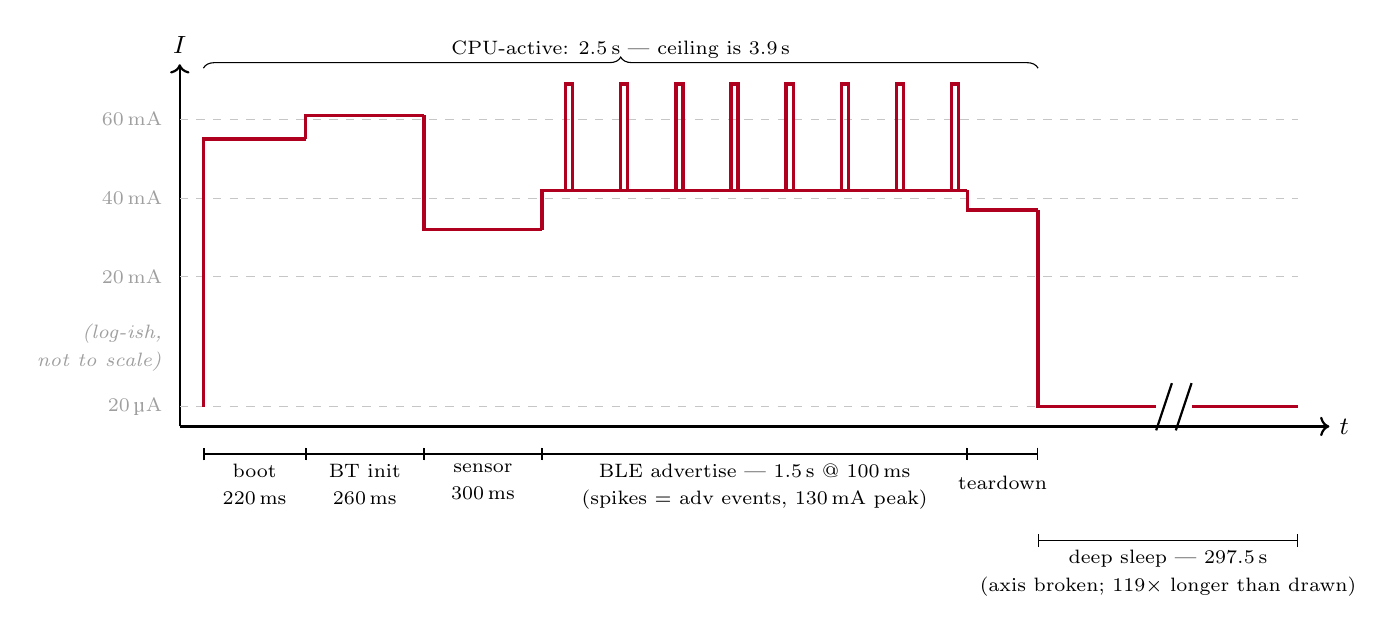
\begin{tikzpicture}[scale=1.0]

  \draw[->,thick] (0,0) -- (14.6,0) node[right]{\small $t$};
  \draw[->,thick] (0,0) -- (0,4.6) node[above]{\small $I$};

  \draw[dashed,gray!45] (0,3.9)  -- (14.2,3.9);  \node[anchor=east,gray!75] at (-0.1,3.9)  {\scriptsize\SI{60}{\milli\ampere}};
  \draw[dashed,gray!45] (0,2.9)  -- (14.2,2.9);  \node[anchor=east,gray!75] at (-0.1,2.9)  {\scriptsize\SI{40}{\milli\ampere}};
  \draw[dashed,gray!45] (0,1.9)  -- (14.2,1.9);  \node[anchor=east,gray!75] at (-0.1,1.9)  {\scriptsize\SI{20}{\milli\ampere}};
  \draw[dashed,gray!45] (0,0.25) -- (14.2,0.25); \node[anchor=east,gray!75] at (-0.1,0.25) {\scriptsize\SI{20}{\micro\ampere}};
  \node[anchor=east,gray!75,align=right] at (-0.1,1.0) {\scriptsize\textit{(log-ish,}\\[-0.7mm]\scriptsize\textit{not to scale)}};

  \draw[very thick,warn] (0.3,0.25) -- (0.3,3.65) -- (1.6,3.65);   % boot 55 mA
  \draw[very thick,warn] (1.6,3.65) -- (1.6,3.95) -- (3.1,3.95);   % BT init 62 mA
  \draw[very thick,warn] (3.1,3.95) -- (3.1,2.50) -- (4.6,2.50);   % sensor 30 mA
  \draw[very thick,warn] (4.6,2.50) -- (4.6,3.00) -- (10.0,3.00);  % adv hold 42 mA
  \foreach \x in {4.9,5.6,6.3,7.0,7.7,8.4,9.1,9.8}{
     \draw[very thick,warn] (\x,3.0) -- (\x,4.35) -- (\x+0.09,4.35) -- (\x+0.09,3.0);
  }
  \draw[very thick,warn] (10.0,3.00) -- (10.0,2.75) -- (10.9,2.75); % teardown 35 mA
  \draw[very thick,warn] (10.9,2.75) -- (10.9,0.25) -- (14.2,0.25); % deep sleep

  \draw[|-|] (0.3,-0.35)  -- (1.6,-0.35)  node[midway,below,align=center]{\scriptsize boot\\[-0.7mm]\scriptsize\SI{220}{\milli\second}};
  \draw[|-|] (1.6,-0.35)  -- (3.1,-0.35)  node[midway,below,align=center]{\scriptsize BT init\\[-0.7mm]\scriptsize\SI{260}{\milli\second}};
  \draw[|-|] (3.1,-0.35)  -- (4.6,-0.35)  node[midway,below,align=center]{\scriptsize sensor\\[-0.7mm]\scriptsize\SI{300}{\milli\second}};
  \draw[|-|] (4.6,-0.35)  -- (10.0,-0.35) node[midway,below,align=center]{\scriptsize BLE advertise --- \SI{1.5}{\second} @ \SI{100}{\milli\second}\\[-0.7mm]\scriptsize (spikes = adv events, \SI{130}{\milli\ampere} peak)};
  \draw[|-|] (10.0,-0.35) -- (10.9,-0.35) node[midway,below,align=center,yshift=-1.5mm]{\scriptsize teardown};
  \draw[|-|] (10.9,-1.45) -- (14.2,-1.45) node[midway,below,align=center]{\scriptsize deep sleep --- \SI{297.5}{\second}\\[-0.7mm]\scriptsize (axis broken; \num{119}$\times$ longer than drawn)};

  \draw[decorate,decoration={brace,amplitude=4pt}] (0.3,4.55) -- (10.9,4.55)
        node[midway,above]{\scriptsize CPU-active: \textbf{\SI{2.5}{\second}} --- ceiling is \SI{3.9}{\second}};

  \draw[white,line width=2.4pt] (12.4,0.25) -- (12.85,0.25);
  \draw[thick] (12.4,-0.05) -- (12.6,0.55);
  \draw[thick] (12.65,-0.05) -- (12.85,0.55);

\end{tikzpicture}
\end{center}

\subsection{Cycle energy, phase by phase (D2)}

\begin{center}
\begin{tabularx}{\textwidth}{Xllll}
\toprule
\textbf{Phase} & \textbf{Duration} & \textbf{$I_\text{mean}$\,\mock} & \textbf{Charge} & \textbf{\% cycle} \\
\midrule
ROM boot + 2nd-stage bootloader (validate skipped)   & \SI{220}{\milli\second}  & \SI{55}{\milli\ampere} & \SI{12.1}{\milli\ampere\second} & \SI{10.6}{\percent} \\
App init + NimBLE controller and host init           & \SI{260}{\milli\second}  & \SI{62}{\milli\ampere} & \SI{16.1}{\milli\ampere\second} & \SI{14.1}{\percent} \\
Sensor read (I\textsuperscript{2}C) + pack + CMAC    & \SI{300}{\milli\second}  & \SI{30}{\milli\ampere} & \SI{9.0}{\milli\ampere\second}  & \SI{7.9}{\percent} \\
BLE non-connectable advertise, \SI{100}{\milli\second} interval, \SI{+9}{\dBm} & \SI{1500}{\milli\second} & \SI{42}{\milli\ampere} & \SI{63.0}{\milli\ampere\second} & \SI{55.3}{\percent} \\
BT teardown + deep-sleep entry                       & \SI{220}{\milli\second}  & \SI{35}{\milli\ampere} & \SI{7.7}{\milli\ampere\second}  & \SI{6.8}{\percent} \\
\midrule
\textbf{CPU-active subtotal} & \textbf{\SI{2.50}{\second}} & \textbf{\SI{43.2}{\milli\ampere}} & \textbf{\SI{107.9}{\milli\ampere\second}} & \textbf{\SI{94.8}{\percent}} \\
Deep sleep                   & \SI{297.5}{\second} & \SI{20}{\micro\ampere} & \SI{5.95}{\milli\ampere\second} & \SI{5.2}{\percent} \\
\midrule
\textbf{Cycle total} & \textbf{\SI{300}{\second}} & \textbf{\SI{380}{\micro\ampere}} & \textbf{\SI{31.6}{\micro\ampere\hour}} & \\
\midrule
\multicolumn{2}{l}{\textit{Annual charge}} & \multicolumn{3}{l}{$\SI{31.6}{\micro\ampere\hour}\times\num{105120} = \SI{3325}{\milli\ampere\hour}$} \\
\multicolumn{2}{l}{\textit{Life on \SI{5100}{\milli\ampere\hour} usable}} & \multicolumn{3}{l}{\textcolor{ok}{\textbf{18.4 months}} --- margin \num{1.53}$\times$} \\
\bottomrule
\end{tabularx}
\end{center}

\medskip
\noindent
\textbf{Read the last column, not the first.} Deep sleep is \SI{99.2}{\percent} of the elapsed time
and \SI{5.2}{\percent} of the energy. The largest single line item is the advertising hold; the
second and third are \emph{boot and initialisation} --- \SI{24.7}{\percent} of the cycle budget
spent before the device has done anything at all. In D3, where the advertising hold is
light-slept away, boot and init become the \textbf{largest} item outright. Optimisation effort
belongs there, not on the radio.

\subsection{D3 --- the literal 30-second window, for comparison}

\begin{center}
\begin{tabularx}{\textwidth}{Xllll}
\toprule
\textbf{Phase} & \textbf{Duration} & \textbf{$I_\text{mean}$\,\mock} & \textbf{Charge} & \textbf{CPU?} \\
\midrule
Boot + bootloader + \SI{32.768}{\kilo\hertz} crystal settle & \SI{420}{\milli\second} & \SI{55}{\milli\ampere} & \SI{23.1}{\milli\ampere\second} & \yes \\
App init + NimBLE init                                      & \SI{260}{\milli\second} & \SI{62}{\milli\ampere} & \SI{16.1}{\milli\ampere\second} & \yes \\
Sensor read + pack                                          & \SI{300}{\milli\second} & \SI{30}{\milli\ampere} & \SI{9.0}{\milli\ampere\second}  & \yes \\
\textbf{Advertising hold --- \SI{500}{\milli\second} interval, automatic light sleep between events} & \SI{30.0}{\second} & \SI{1.9}{\milli\ampere} & \SI{57.0}{\milli\ampere\second} & \no \\
Teardown + deep-sleep entry                                 & \SI{220}{\milli\second} & \SI{35}{\milli\ampere} & \SI{7.7}{\milli\ampere\second}  & \yes \\
\midrule
\textbf{Awake subtotal} & \textbf{\SI{31.2}{\second}} & \textbf{\SI{3.6}{\milli\ampere}} & \textbf{\SI{112.9}{\milli\ampere\second}} & \\
Deep sleep              & \SI{268.8}{\second} & \SI{20}{\micro\ampere} & \SI{5.4}{\milli\ampere\second} & \\
\midrule
\textbf{Cycle total} & \textbf{\SI{300}{\second}} & \textbf{\SI{394}{\micro\ampere}} & \textbf{\SI{32.9}{\micro\ampere\hour}} & \\
\midrule
\multicolumn{2}{l}{\textit{Life on \SI{5100}{\milli\ampere\hour} usable}} & \multicolumn{3}{l}{\textcolor{ok}{\textbf{17.7 months}} --- margin \num{1.48}$\times$} \\
\bottomrule
\end{tabularx}
\end{center}

\noindent
The \SI{30}{\second} advertising hold costs \SI{57}{\milli\ampere\second}; D2's
\SI{1.5}{\second} hold costs \SI{63}{\milli\ampere\second}. \textbf{They cost the same.} A
\num{20}$\times$ longer window at \num{22}$\times$ lower current is a wash. \textbf{So the choice
between D2 and D3 is not a power decision at all} --- decide it on these grounds instead:

\begin{center}
\begin{tabularx}{\textwidth}{lXX}
\toprule
& \textbf{D2 --- short window} & \textbf{D3 --- literal \SI{30}{\second}} \\
\midrule
BOM       & No extra parts. & \textbf{Requires a \SI{32.768}{\kilo\hertz} crystal} for the BT low-power clock. \\
Firmware  & Simple. No \texttt{esp\_pm}, no tickless idle, no BT modem sleep. & Needs \texttt{CONFIG\_PM\_ENABLE}, tickless idle and BT modem sleep, all interacting. The hardest class of bug to find. \\
Gateway   & \SI{1.5}{\second} to catch \num{15} adv events. Needs a \emph{continuously} scanning gateway. & \SI{30}{\second} window, \num{60} adv events. Tolerant of a gateway that scans intermittently, or round-robins across many nodes. \\
Reception margin & Lower. A gateway busy elsewhere for \SI{1.5}{\second} misses the cycle entirely. & \textbf{High. This is D3's real justification.} \\
\bottomrule
\end{tabularx}
\end{center}

\noindent
Choose \textbf{D2} if the gateway scans continuously and serves few nodes. Choose \textbf{D3} if
one gateway must round-robin across many nodes, or if the \SI{30}{\second} window is contractual.
\emph{Do not choose between them on battery life --- there is nothing to choose.}

\medskip
\noindent
\fcolorbox{warn}{white}{\parbox{0.97\textwidth}{%
\textbf{The two paths have different BOMs. Decide before the board is laid out.} D2 wants
\emph{no} \SI{32.768}{\kilo\hertz} crystal --- fitting one costs roughly \SI{200}{\milli\second}
of startup on \emph{every} wake, which is \SI{10}{\percent} of D2's entire CPU-active budget, to
buy a timing accuracy the design does not need. D3 cannot work without one. Retrofitting the
crystal later is a board spin; omitting it later is not.}}

% ---------------------------------------------------------------------------
\section{Energy cost of each nff operation}
\label{sec:tools}

Mock values\,\mock. Energy is reported at the module's \SI{3.3}{\volt} rail
($E = \SI{3.3}{\volt}\cdot I\cdot t$), which is the quantity a battery design cares about. The rig
in \texttt{datasheet.tex} measures the whole devkit at its \SI{5}{\volt} input and must be
de-embedded before its figures can be substituted here.

\subsection{Steady-state and command operations}

\begin{center}
\begin{tabularx}{\textwidth}{Xlllc}
\toprule
\textbf{Operation} & \textbf{Duration} & \textbf{$I_\text{mean}$} & \textbf{Energy} & \textbf{Radio} \\
\midrule
\texttt{nff\_init()} --- NVS read, panic hook, OTA boot-check & \SI{12}{\milli\second} & \SI{40}{\milli\ampere} & \SI{1.6}{\milli\joule} & --- \\
WiFi associate + DHCP \meas                                    & \SI{3.1}{\second}       & \SI{64.7}{\milli\ampere}& \SI{662}{\milli\joule} & TX/RX \\
SNTP time sync \emph{(cold boot; hardcoded)}                   & \SI{1.8}{\second}       & \SI{95}{\milli\ampere} & \SI{564}{\milli\joule} & TX/RX \\
\texttt{nff\_connect()} --- mTLS handshake, MQTT CONNECT, SUBSCRIBE & \SI{1.6}{\second}  & \SI{110}{\milli\ampere}& \SI{581}{\milli\joule} & TX/RX \\
Heartbeat publish (QoS\,1 retained, 250-byte JSON)             & \SI{45}{\milli\second}  & \SI{120}{\milli\ampere}& \SI{17.8}{\milli\joule}& TX \\
MQTT keepalive \texttt{PINGREQ}                                & \SI{12}{\milli\second}  & \SI{115}{\milli\ampere}& \SI{4.6}{\milli\joule} & TX/RX \\
\texttt{nff\_loop()} idle tick (connected, no work)            & \SI{0.4}{\milli\second} & \SI{38}{\milli\ampere} & \SI{0.05}{\milli\joule}& --- \\
\texttt{nff\_log()} one line (UART + RTC ring)                 & \SI{0.3}{\milli\second} & \SI{42}{\milli\ampere} & \SI{0.04}{\milli\joule}& --- \\
\midrule
Inbound command: ECDSA-P256 verify \emph{(CPU-bound)}          & \SI{55}{\milli\second}  & \SI{62}{\milli\ampere} & \SI{11.3}{\milli\joule}& --- \\
\quad$\hookrightarrow$ \texttt{ping} response                  & \SI{18}{\milli\second}  & \SI{118}{\milli\ampere}& \SI{7.0}{\milli\joule} & TX \\
\quad$\hookrightarrow$ \texttt{diag} response (heap + RSSI)    & \SI{30}{\milli\second}  & \SI{118}{\milli\ampere}& \SI{11.7}{\milli\joule}& TX \\
\quad$\hookrightarrow$ \texttt{reboot} (ack + restart)         & \SI{0.9}{\second}       & \SI{88}{\milli\ampere} & \SI{261}{\milli\joule} & TX \\
\midrule
Crash report publish (2.5\,kB retained) + NVS erase            & \SI{180}{\milli\second} & \SI{105}{\milli\ampere}& \SI{62}{\milli\joule}  & TX \\
Reconnect attempt --- one failed TLS handshake                 & \SI{1.9}{\second}       & \SI{108}{\milli\ampere}& \SI{677}{\milli\joule} & TX/RX \\
Bootstrap announce + cert rollover (chunked NVS writes)        & \SI{3.2}{\second}       & \SI{112}{\milli\ampere}& \SI{1.18}{\joule}      & TX/RX \\
\bottomrule
\end{tabularx}
\end{center}

\subsection{OTA --- the dominant single operation}

\begin{center}
\begin{tabularx}{\textwidth}{Xllll}
\toprule
\textbf{OTA phase} (1.2\,MB image) & \textbf{Duration} & \textbf{$I_\text{mean}$} & \textbf{Energy} & \textbf{Charge} \\
\midrule
Command verify (ECDSA, nonce ring, anti-downgrade)  & \SI{55}{\milli\second} & \SI{62}{\milli\ampere}  & \SI{11.3}{\milli\joule} & --- \\
\texttt{ota\_started} publish                       & \SI{40}{\milli\second} & \SI{120}{\milli\ampere} & \SI{15.8}{\milli\joule} & --- \\
HTTP GET stream + flash write (4\,kB chunks) \meas & \SI{9.8}{\second}    & \SI{150.5}{\milli\ampere} & \SI{4.89}{\joule}       & \SI{0.41}{\milli\ampere\hour} \\
NVS commit (\texttt{ota\_trial}) + reboot           & \SI{0.7}{\second}      & \SI{90}{\milli\ampere}  & \SI{208}{\milli\joule}  & --- \\
\midrule
\textbf{OTA download total} \meas & \textbf{\SI{9.9}{\second}} & \textbf{\SI{150}{\milli\ampere}} & \textbf{\SI{4.92}{\joule}} & \textbf{\SI{0.41}{\milli\ampere\hour}} \\
\midrule
Probation soak (\texttt{NFF\_OTA\_MIN\_HEALTHY\_MS} = \SI{5000}{\milli\second}) & \SI{5.0}{\second} & \SI{82}{\milli\ampere} & \SI{1.35}{\joule} & \SI{0.11}{\milli\ampere\hour} \\
Rollback (partition switch, reboot, \texttt{ota\_result})                        & \SI{0.9}{\second} & \SI{88}{\milli\ampere} & \SI{261}{\milli\joule} & --- \\
\bottomrule
\end{tabularx}
\end{center}

\noindent
An OTA costs \SI{0.41}{\milli\ampere\hour} --- \SI{0.007}{\percent} of the battery \meas. \textbf{OTA is
not the problem.} A device could take an update every week for its entire life and spend under
\SI{1}{\percent} of its energy on it. It is the \emph{recurring} costs that kill it.

\subsection{Why WiFi was never an option}

\begin{center}
\begin{tabularx}{\textwidth}{Xlll}
\toprule
\textbf{Recurring cost, as the nff SDK ships} & \textbf{Per event} & \textbf{Events/yr} & \textbf{Annual charge} \\
\midrule
Heartbeat, \texttt{heartbeat\_interval\_s} = \num{30} (default)      & \SI{1.5}{\micro\ampere\hour} & \num{1051200} & \SI{1577}{\milli\ampere\hour} \\
Heartbeat, \texttt{heartbeat\_interval\_s} = \num{300} (Kconfig max) & \SI{1.5}{\micro\ampere\hour} & \num{105120}  & \SI{158}{\milli\ampere\hour} \\
\midrule
\textbf{WiFi associated + idle} \emph{(the SDK never enables WiFi power save)} & --- & continuous & \textcolor{warn}{$\approx$\SI{876000}{\milli\ampere\hour}} \\
\bottomrule
\end{tabularx}
\end{center}

\noindent
\fcolorbox{warn}{white}{\parbox{0.97\textwidth}{%
\textbf{An nff device on WiFi, exactly as the SDK ships, lasts 2.5 days on this battery.} The
default heartbeat alone spends \SI{26}{\percent} of a \SI{6000}{\milli\ampere\hour} cell per year
--- and that is only the \emph{publishes}. The association that carries them holds the radio at
roughly \SI{100}{\milli\ampere} continuously, because \texttt{nff-sdk-c} never calls
\texttt{esp\_wifi\_set\_ps()}. Even with WiFi power save and DTIM\,3 --- which would have to be
added --- an always-associated station averages roughly \SI{7}{\milli\ampere}, giving
\textbf{36 days}. \emph{The BLE-only decision in the requirement is not a preference. It is the
only transport that can meet this budget, and it was the right call.}}}

% ---------------------------------------------------------------------------
\section{Where the nff SDK actually stands}
\label{sec:sdk}

\subsection{Two structural gaps}

\noindent
\fcolorbox{warn}{white}{\parbox{0.97\textwidth}{%
\textbf{\texttt{nff-sdk-c} cannot run on this device today.} Not ``needs tuning'' --- cannot run.
Two gaps, both established by reading the source rather than inferred:

\medskip
\textbf{1. There is no BLE.} \texttt{include/nff\_port.h} is the SDK's \emph{only} hardware
contract (``all nine SDK modules call only \texttt{nff\_port\_*} functions''). Its transport
entries are \texttt{nff\_port\_mqtt\_*} (MQTT over mTLS) and
\texttt{nff\_port\_https\_get\_stream} (HTTPS, for OTA). There is no \texttt{nff\_port\_ble\_*}. A
repository-wide search for \texttt{BLE}, \texttt{NimBLE}, \texttt{bluedroid},
\texttt{esp\_bt\_*}, \texttt{esp\_ble\_*}, \texttt{gatt} and \texttt{advertis*} returns
\textbf{zero hits in any firmware source}. (\texttt{nff\_crash.c}'s \texttt{bt\_json} is a
\emph{backtrace}; \texttt{nff-pentester/.../ble.py} is a host-side Python tool.)

\medskip
\textbf{2. There is no sleep.} No \texttt{esp\_deep\_sleep}, \texttt{esp\_light\_sleep},
\texttt{esp\_sleep\_enable\_*}, \texttt{esp\_pm\_*}, \texttt{WIFI\_PS\_*} or
\texttt{rtc\_gpio\_*} anywhere in \texttt{nff-sdk-c/}. \texttt{nff\_loop()} presumes a
continuously-associated station, and the fleet marks a device offline after
$2\times$\texttt{heartbeat\_interval\_s} of silence --- i.e.\ the protocol is \emph{built on} the
assumption that the device is always reachable. The SDK's entire low-power story is one sentence
in \texttt{docs/PROTOCOL.md}: raise \texttt{heartbeat\_interval\_s}.}}

\subsection{Settings that do apply}

\begin{center}
\begin{tabularx}{\textwidth}{llX}
\toprule
\textbf{Symbol} & \textbf{Default $\rightarrow$ set} & \textbf{Why} \\
\midrule
\texttt{cfg.heartbeat\_interval\_s} \newline \texttt{CONFIG\_NFF\_HEARTBEAT\_INTERVAL\_S}
  & $30 \rightarrow \mathbf{300}$
  & The only shipped power knob, and \num{300} is the Kconfig ceiling. It aligns the heartbeat to
    the \SI{5}{\minute} wake cycle: \textbf{one heartbeat per wake, and none in between}. \\
\texttt{NFF\_MQTT\_BUFFER\_SIZE}
  & $1024 \rightarrow \mathbf{1024}$
  & \textbf{Not a power knob --- a landmine.} The OTA command is roughly 420 bytes;
    PubSubClient's 256-byte default \emph{silently drops} it. Shrinking this to reclaim RAM breaks
    OTA with no error anywhere. Leave it alone. \\
\texttt{NFF\_TIMESTAMP\_WINDOW\_S}
  & $300 \rightarrow \mathbf{3600}$
  & Commands are replay-guarded against an SNTP-set RTC within $\pm\SI{300}{\second}$. A
    duty-cycled device has no SNTP, and its RTC runs on the internal \SI{150}{\kilo\hertz} RC
    ($\pm\SI{5}{\percent}$ --- $\pm\SI{15}{\second}$ per \SI{5}{\minute} cycle, unbounded across
    sleeps). At \num{300} it will start rejecting valid commands. \\
\texttt{NFF\_LOG\_LINES} $\times$ \texttt{NFF\_LOG\_LINE\_LEN}
  & $32\times128 \rightarrow \mathbf{8\times96}$
  & The ring lives in \texttt{RTC\_NOINIT}, which is \emph{retained through deep sleep} and
    therefore costs standby current. Trim it; do not remove it --- it is the crash-report path. \\
\texttt{NFF\_OTA\_MAX\_DL\_RETRIES}
  & $4 \rightarrow \mathbf{2}$
  & Each retry is a fresh TLS handshake plus a ranged resume. On battery, a failing OTA should die
    fast and retry next cycle rather than grind. \\
\texttt{NFF\_OTA\_CONFIRM\_TIMEOUT\_S} \newline \texttt{NFF\_OTA\_MIN\_HEALTHY\_MS}
  & $60,\ 5000 \rightarrow$ \textbf{unchanged}
  & \textbf{Do not shorten either.} A duty-cycled device only reaches its health checks while
    awake; a short probation would roll back a perfectly good image. Note the consequence:
    \SI{5}{\second} of \emph{continuous} healthy soak \emph{exceeds the \SI{3.9}{\second}
    CPU-active ceiling} on its own --- so an OTA-probation cycle is necessarily a long-wake
    exception. Budget one (\S\ref{sec:params}). \\
\bottomrule
\end{tabularx}
\end{center}

\subsection{Two hardcoded behaviours that must become configurable}

\noindent
\fcolorbox{warn}{white}{\parbox{0.97\textwidth}{%
\textbf{The reconnect backoff ladder is the SDK's worst battery failure mode, and it is not a
setting.} \texttt{nff\_core.c:31} hardcodes
\texttt{\{1000, 2000, 4000, 8000, 16000, 32000, 60000\}}\,\si{\milli\second}, \emph{saturating at
\SI{60}{\second}}. A device that cannot reach its peer therefore retries forever, once a minute,
and each retry is a full radio bring-up plus a TLS handshake --- about \SI{677}{\milli\joule}, or
\SI{57}{\micro\ampere\hour}. That is \SI{500}{\milli\ampere\hour} per month, \textbf{with no
telemetry to show for it}, while the fleet sees only a device that has gone dark. It must be
capped, and it must be able to give up and go back to sleep.

\medskip
\textbf{SNTP is unconditional, and it blocks \texttt{nff\_connect()}.}
\texttt{nff\_port\_esp32\_arduino.c:60} hardcodes
\texttt{configTime(0, 0, "pool.ntp.org", \ldots)} and polls for up to roughly \SI{20}{\second} on
a cold boot with an unset RTC --- mTLS is \emph{skipped} until it lands. A duty-cycled device
cold-boots \emph{every cycle}. As written, this would spend \SI{20}{\second} on NTP per wake:
\textbf{five times the entire CPU-active budget}, on a service the device does not need.}}

\subsection{Required SDK work}

\begin{center}
\begin{tabularx}{\textwidth}{lX}
\toprule
\textbf{Addition} & \textbf{Notes} \\
\midrule
\texttt{nff\_port\_ble\_adv\_start} / \texttt{\_stop} / \texttt{\_set\_payload} / \texttt{\_set\_tx\_power}
  & New entries in \texttt{nff\_port.h}. \textbf{The good news: this is an addition, not a
    rewrite.} The PAL is already the sole hardware contract, so a BLE port slots in beside the
    MQTT one without touching the nine core modules. \\
\texttt{nff\_port\_sleep\_deep(ms)} / \texttt{nff\_port\_sleep\_light(ms)}
  & New. Nothing in the PAL touches power today. \\
\texttt{nff\_run\_once()} --- do work, return
  & Beside \texttt{nff\_loop()} / \texttt{nff\_start\_task()}. The latter pins an 8\,kB,
    priority-2 FreeRTOS task to Core\,0 that \emph{never exits} --- structurally the wrong shape
    for a device whose whole job is to reach deep sleep. \\
State retained across deep sleep
  & \textbf{The mechanism already exists.} \texttt{nff\_crash.c} keeps its log ring in
    \texttt{RTC\_NOINIT}. Reuse it for \texttt{seq}, backoff state and OTA trial state, so that a
    cold boot every cycle is not a \emph{cold} boot. \\
Packed 27-byte heartbeat codec
  & The heartbeat is a 250-byte JSON (\texttt{char payload[416]},
    \texttt{nff\_heartbeat.c:38}). A BLE 4.2 legacy advertisement carries 31 bytes \emph{total}.
    It does not fit, and it cannot be made to fit --- see \S\ref{sec:adv}. \\
Gateway-side MQTT bridge
  & The gateway holds the mTLS identity and republishes to
    \texttt{nff/\{project\}/devices/\{id\}/heartbeat}. The device's ECDSA-verified command path
    (\texttt{nff\_cmd.c}) must move to a BLE GATT write, or be dropped. \\
OTA over BLE
  & \texttt{nff\_port\_https\_get\_stream} has no BLE analogue. 1.2\,MB over BLE 4.2 1M PHY (there
    is \textbf{no LE 2M PHY} on this part --- \S\ref{sec:params}) at a realistic 15\,kB/s is about
    \SI{80}{\second} of connected radio, or \SI{2.5}{\milli\ampere\hour}. Affordable as a rare
    event. But it is a \emph{connection}, not an advertisement, and none of that code exists. \\
\bottomrule
\end{tabularx}
\end{center}

% ---------------------------------------------------------------------------
\section{ESP32 and BLE parameters}
\label{sec:params}

\subsection{What the WROOM-32E can and cannot do}

\begin{center}
\begin{tabularx}{\textwidth}{clX}
\toprule
& \textbf{Capability} & \textbf{Consequence} \\
\midrule
\yes & Bluetooth 4.2, BR/EDR + BLE & BLE works. BR/EDR is dead weight --- compile it out. \\
\yes & Deep sleep, RTC-timer wake, $\approx\SI{10}{\micro\ampere}$ (module) & Covers the \SI{4.5}{\minute} of every cycle. \\
\yes & Light sleep, $\approx\SI{0.8}{\milli\ampere}$ & This is what makes D3 possible. \\
\midrule
\no  & \textbf{Extended advertising} & \textbf{You get 31 bytes of advertising payload, not 255.} Extended advertising is a BT\,5.0 feature. If any part of the payload design assumed otherwise, it breaks here. \\
\no  & LE 2M PHY & All BLE traffic, including any future OTA, runs at 1M. \\
\no  & LE Coded PHY (long range) & Range must be bought with TX power, not with coding gain. \\
\bottomrule
\end{tabularx}
\end{center}

\medskip
\noindent
\fcolorbox{ok}{white}{\parbox{0.97\textwidth}{%
\textbf{If one part can still be changed, change this one.} An ESP32-C3-MINI-1 or ESP32-C6 is the
same price class and footprint class, and gives BLE 5.0 --- extended advertising (255-byte
payloads, so the nff heartbeat would fit \emph{as-is}), LE 2M PHY, and Coded PHY for range --- at
roughly \emph{half} the active current. The WROOM-32E's dual Xtensa cores and BR/EDR radio are
pure liability in a device whose entire job is to wake, read one sensor, and go back to sleep.
\emph{The design closes on the WROOM-32E anyway} --- at \num{1.5}$\times$ margin instead of
roughly \num{3}$\times$. This is a recommendation, not a blocker.}}

\subsection{Recommended configuration}

\begin{center}
\begin{tabularx}{\textwidth}{lllX}
\toprule
\textbf{Setting} & \textbf{D2} & \textbf{D3} & \textbf{Why} \\
\midrule
\texttt{CONFIG\_BT\_NIMBLE\_ENABLED} & \multicolumn{2}{l}{\texttt{y}} & NimBLE over Bluedroid: about 60\,kB less RAM and a materially shorter init. \textbf{Init is on the critical path --- it runs every cycle}, and it is \SI{14}{\percent} of the D2 budget. \\
\texttt{CONFIG\_BT\_CLASSIC\_ENABLED} & \multicolumn{2}{l}{\texttt{n}} & BR/EDR is unused; leaving it in costs init time and RAM. \\
WiFi & \multicolumn{2}{l}{\textbf{never initialised}} & Do not call \texttt{WiFi.begin()} / \texttt{esp\_wifi\_init()}. An \emph{initialised but idle} WiFi stack holds the RF and PLL power domains up. This is the single easiest way to silently lose the entire budget. \\
\texttt{CONFIG\_BOOTLOADER\_SKIP\_VALIDATE\_IN\_DEEP\_SLEEP} & \multicolumn{2}{l}{\texttt{y}} & Skips the app-image SHA-256 check on a deep-sleep wake. Saves \SIrange{100}{200}{\milli\second} \emph{every cycle} --- \SIrange{2}{3}{\percent} of the whole energy budget, for one config flag. \\
\texttt{CONFIG\_BOOTLOADER\_LOG\_LEVEL} & \multicolumn{2}{l}{\texttt{NONE}} & Bootloader UART chatter is pure cost on a battery. \\
\texttt{CONFIG\_LOG\_DEFAULT\_LEVEL} & \multicolumn{2}{l}{\texttt{ERROR}} & \texttt{nff\_log()} writes UART unconditionally; the cost is the CPU time to \texttt{printf}-format, not the UART itself. \\
\texttt{CONFIG\_ESP32\_DEFAULT\_CPU\_FREQ\_MHZ} & \multicolumn{2}{l}{\texttt{80}} & The wake window is dominated by \emph{waiting} --- for the sensor, for adv events --- not by computing. Race-to-idle does not pay when there is nothing to race. \\
\texttt{CONFIG\_ESP32\_RTC\_CLK\_SRC} & \texttt{INT\_RC} & \texttt{EXT\_CRYS} & \textbf{The BOM fork.} D2: no crystal --- it costs roughly \SI{200}{\milli\second} of startup per wake and buys an accuracy the design does not need. D3: mandatory, for the BT low-power clock. \\
\texttt{CONFIG\_PM\_ENABLE} \newline \texttt{CONFIG\_FREERTOS\_USE\_TICKLESS\_IDLE} \newline \texttt{CONFIG\_BTDM\_CTRL\_MODEM\_SLEEP} & \texttt{n} & \texttt{y} & The three settings that make D3 work: together they let the BT controller hold advertising timing while the CPU is in light sleep. \textbf{All three, or none} --- any one of them missing and the CPU simply stays awake, silently, and you have built D1. \\
\midrule
Advertising type & \multicolumn{2}{l}{\texttt{ADV\_NONCONN\_IND}} & \textbf{Non-connectable \emph{and} non-scannable.} A connectable or scannable advertisement forces the receiver on after every advertising packet, to listen for a \texttt{SCAN\_REQ} that will never come --- roughly doubling radio energy for a device that has nothing to say back. \\
Advertising interval & \SI{100}{\milli\second} & \SI{500}{\milli\second} & D2: \num{15} events in \SI{1.5}{\second}. D3: \num{60} events in \SI{30}{\second}, sparse enough that light sleep gets a real duty cycle in between. \\
TX power & \multicolumn{2}{l}{\textbf{\SI{+9}{\dBm}}} & See the box below. \\
BLE address & \multicolumn{2}{l}{static random, \textbf{fixed}} & \emph{Not} a rotating RPA. The gateway keys deduplication on the address, and the address \emph{is} the device's identity --- which is why the payload need not spend bytes carrying one (\S\ref{sec:adv}). \\
\bottomrule
\end{tabularx}
\end{center}

\medskip
\noindent
\fcolorbox{ok}{white}{\parbox{0.97\textwidth}{%
\textbf{Spend the link margin. Set TX power to \SI{+9}{\dBm}, the maximum.} This is
counterintuitive, and it is correct. The radio is on for roughly \SI{2.5}{\milli\second} of each
\SI{100}{\milli\second} advertising interval --- a \SI{2.5}{\percent} duty cycle, inside a phase
that is itself \SI{0.5}{\percent} of the wall-clock cycle. Raising TX power from \SI{0}{\dBm} to
\SI{+9}{\dBm} moves the \emph{cycle} budget by well under \SI{1}{\percent}. A \emph{missed}
advertisement, by contrast, costs a whole wasted cycle --- about \SI{30}{\micro\ampere\hour}, or
\SI{60}{\percent} of a cycle's entire budget, plus the lost reading. \textbf{The arithmetic says
buy range with power and never think about it again.} The instinct to turn the radio down to save
battery is, on this design, exactly backwards.}}

\subsection{Budget the exception cycles}

Three cycles are not like the others, and a design that budgets only the nominal cycle will drift.

\begin{center}
\begin{tabularx}{\textwidth}{lllX}
\toprule
\textbf{Exception} & \textbf{Cost} & \textbf{Budget} & \textbf{Notes} \\
\midrule
OTA probation soak & \SI{0.11}{\milli\ampere\hour} & 12/yr & \texttt{NFF\_OTA\_MIN\_HEALTHY\_MS} = \SI{5}{\second} of \emph{continuous} healthy soak exceeds the \SI{3.9}{\second} CPU-active ceiling on its own. Accept it as a long-wake exception; do not shorten the soak to make it fit. \\
OTA download & \SI{1.89}{\milli\ampere\hour} & 12/yr & \SI{23}{\milli\ampere\hour} per year --- \SI{0.4}{\percent} of the battery. Negligible. \\
Crash report & \SI{0.02}{\milli\ampere\hour} & rare & Negligible. \\
\midrule
\textbf{Unreachable gateway} & \textcolor{warn}{\SI{57}{\micro\ampere\hour} \textbf{per retry}} & \textcolor{warn}{\textbf{unbounded}} & \textbf{The only exception that matters.} Per \S\ref{sec:sdk}, the backoff ladder saturates at one full radio bring-up per minute, forever. Cap it, or a single dead gateway drains a \SI{6000}{\milli\ampere\hour} node in weeks. \\
\bottomrule
\end{tabularx}
\end{center}

% ---------------------------------------------------------------------------
\section{The 31-byte advertisement}
\label{sec:adv}

BLE 4.2 legacy advertising carries 31 bytes of \texttt{AdvData}. One Manufacturer Specific Data
structure costs 4 bytes of framing (length, type \texttt{0xFF}, and a 2-byte company identifier),
leaving \textbf{27 bytes} of payload.

\begin{center}
\begin{tabularx}{\textwidth}{llX}
\toprule
\textbf{Field} & \textbf{Bytes} & \textbf{Notes} \\
\midrule
\textit{(AD framing: length, \texttt{0xFF}, company ID)} & \textit{4} & \textit{Not payload.} \\
\midrule
\texttt{ver} / packet type & 1  & Lets the codec evolve without a fleet-wide flag day. \\
\texttt{seq}               & 2  & Wraps. The gateway deduplicates on (address, seq) --- \num{15} adv events per wake are \num{15} copies of \emph{one} reading, not \num{15} readings. \\
\texttt{flags}             & 1  & Status, OTA trial state, low battery. \\
\texttt{fw\_build\_id}     & 2  & Enough for the fleet to see what is actually deployed. \\
\texttt{battery}           & 1  & Percent. \\
\textbf{sensor payload}    & \textbf{16} & \textbf{What is left --- and it is the entire point of the device.} \\
\texttt{tag}               & 4  & AES-CMAC-128, truncated. Prevents a spoofed reading; does \emph{not} give confidentiality. \\
\midrule
\textbf{Total} & \textbf{27} & \textbf{= the payload ceiling. Exactly full.} \\
\bottomrule
\end{tabularx}
\end{center}

\begin{description}[style=nextline,leftmargin=0pt]
  \item[The device identity is free --- do not pay for it twice.] The 6-byte static random BLE
        address is already in the advertising packet header. Spending payload bytes on a device ID
        would take a quarter of the sensor field to carry information the gateway already has.
  \item[The nff heartbeat does not fit, by \num{8}$\times$.] It is a 250-byte JSON
        (\texttt{char payload[416]}, \texttt{nff\_heartbeat.c:38}). No compression story closes an
        \num{8}$\times$ gap. The gateway must \emph{reconstruct} the JSON heartbeat from the
        packed 27-byte record and publish it to the fleet --- which is also where the mTLS
        identity and the SNTP-correct timestamp come from.
\end{description}

\medskip
\noindent
\fcolorbox{warn}{white}{\parbox{0.97\textwidth}{%
\textbf{The Flags AD structure will silently eat 3 of your 27 bytes if you let it.} Flags is only
\emph{required} for a discoverable device; a non-connectable beacon may omit it. NimBLE emits
exactly the AD structures you hand it. Bluedroid's \texttt{esp\_ble\_gap\_config\_adv\_data()}
helper \textbf{inserts Flags for you} --- use \texttt{esp\_ble\_gap\_config\_adv\_data\_raw()}
instead. Get this wrong and the sensor field silently shrinks from 16 bytes to 13, which is the
kind of thing that gets discovered after the enclosure tooling is cut.}}

% ---------------------------------------------------------------------------
\section{The sleep floor is a board property, not a chip property}
\label{sec:sleep}

\begin{center}
\begin{tabularx}{\textwidth}{Xll}
\toprule
& \textbf{Custom board} & \textbf{Devkit} \\
\midrule
ESP32-WROOM-32E, deep sleep, RTC timer only & \SI{10}{\micro\ampere} & \SI{10}{\micro\ampere} \\
LDO quiescent & \SI{1.6}{\micro\ampere}\ \footnotesize(MCP1700 class) & \textcolor{warn}{\SI{5000}{\micro\ampere}}\ \footnotesize(AMS1117) \\
USB--UART bridge & --- \footnotesize(not fitted) & \textcolor{warn}{\SI{100}{\micro\ampere}}\ \footnotesize(CP2102) \\
Power LED & --- \footnotesize(not fitted) & \textcolor{warn}{\SI{1400}{\micro\ampere}} \\
Sensor(s), standby & \SI{3}{\micro\ampere} & \SI{3}{\micro\ampere} \\
Leakage, pull-ups, RTC\_SLOW retention & \SI{5}{\micro\ampere} & \SI{5}{\micro\ampere} \\
\midrule
\textbf{Total sleep floor} & \textbf{\SI{20}{\micro\ampere}} & \textcolor{warn}{\textbf{\SI{6.5}{\milli\ampere}}} \\
\textbf{Sleep alone, vs.\ the \SI{582}{\micro\ampere} budget} & \SI{3.4}{\percent} & \textcolor{warn}{\textbf{\num{11}$\times$ over}} \\
\bottomrule
\end{tabularx}
\end{center}

\noindent
\fcolorbox{warn}{white}{\parbox{0.97\textwidth}{%
\textbf{A devkit fails the requirement while doing nothing at all.} Its \SI{5}{\milli\ampere}
AMS1117 and its power LED draw more, asleep, than the entire per-cycle budget. No firmware can
recover this. \textbf{Any battery-life number measured on a devkit is meaningless.}

\medskip
And this is precisely the trap the shunt rig's own datasheet describes --- in reverse. That rig
deliberately measures the \emph{whole devkit board}, LDO and bridge and LED included, because for
\emph{its} purpose (the marginal energy of an OTA) those terms are constant and cancel.
\emph{Here they do not cancel. Here they are the answer.}}}

% ---------------------------------------------------------------------------
\section{Battery: \si{\milli\ampere\hour} is not the binding constraint}
\label{sec:battery}

The \SI{85}{\percent} derate used in \S\ref{sec:verdict} is not a fudge factor. It is a stand-in
for four separate effects, and each must be checked against the actual cell.

\begin{center}
\begin{tabularx}{\textwidth}{lX}
\toprule
\textbf{Effect} & \textbf{What to check} \\
\midrule
Self-discharge & Chemistry-dependent, and \emph{not} small over 12 months. Li-SOCl$_2$: about \SI{1}{\percent} per year. Li-ion: \SIrange{2}{3}{\percent} \emph{per month} --- which alone would consume \SIrange{24}{36}{\percent} of the pack over the target life. \textbf{The chemistry choice is a \SI{30}{\percent} swing in the budget.} \\
Low temperature & Capacity falls with temperature, and the sites are presumably not climate-controlled. Derate against the coldest expected ambient, not the datasheet's \SI{25}{\celsius}. \\
Cut-off voltage & The ESP32's radio needs a solid $\geq\SI{3.0}{\volt}$. From a \SI{3.6}{\volt} Li-SOCl$_2$ cell, an LDO has almost no headroom by end of life; a buck-boost may be required --- and then its own efficiency and quiescent current enter the budget. \\
\midrule
\textbf{Pulse capability} & \textbf{See below. This is the one that bites.} \\
\bottomrule
\end{tabularx}
\end{center}

\noindent
\fcolorbox{warn}{white}{\parbox{0.97\textwidth}{%
\textbf{The battery's ability to source \SI{130}{\milli\ampere} pulses matters more than its
\si{\milli\ampere\hour} rating.} Li-SOCl$_2$ cells --- the obvious chemistry for a 12-month,
\SI{6000}{\milli\ampere\hour}, low-average-current design --- have high internal impedance and
\emph{passivate} during long idle periods. The consequences are specific, and they all land on
this design:

\medskip
\begin{itemize}[leftmargin=*,nosep]
  \item The roughly \SI{250}{\milli\ampere} boot inrush and the roughly \SI{130}{\milli\ampere}
        BLE TX pulse will sag the terminal voltage.
  \item \textbf{The worst pulse is the first one after a long idle} --- which is exactly the pulse
        this design takes, every cycle, forever. A brownout there is a boot loop, and a boot loop
        on this battery is a dead device within days.
  \item A design that passes on the bench with a fresh cell can still fail in the field at month
        nine, as internal impedance rises with depth of discharge.
\end{itemize}

\medskip
\textbf{Mitigation:} a hybrid layer capacitor (HLC), or a supercapacitor with a series limiting
resistor across the cell, sized for the boot inrush. \textbf{Verification:} scope the rail during
the \emph{first} advertising event after an hour of deep sleep, on a \emph{partially-discharged}
cell. Not a fresh one --- and not a bench supply, which will pass this test every time and tell
you nothing.}}

% ---------------------------------------------------------------------------
\section{How this budget can lie to you}
\label{sec:lie}

In the spirit of the rig's own honesty section: each of these is a way to arrive at a confident,
plausible, \emph{wrong} answer.

\begin{enumerate}[leftmargin=*,label=\textbf{L\arabic*.}]
  \item \textbf{Every number in this document is a mock.}\ \mock\ Nothing here is measured. The
        arithmetic is sound, and the \emph{ratios} are the point --- a \num{27}$\times$ spread
        between D0 and D2 does not collapse to \num{1}$\times$ if the currents turn out to be
        \SI{30}{\percent} off. But do not quote an absolute month figure to a customer from this
        revision.

  \item \textbf{The existing rig cannot measure the most important number here.} Its own datasheet
        says so: deep sleep at \SI{10}{\micro\ampere} across a \SI{1}{\ohm} shunt is
        \SI{10}{\micro\volt}, roughly \num{100}$\times$ below the breadboard noise floor, and its
        capability envelope marks deep sleep \no. \textbf{Every sleep-current figure in this
        document is unmeasurable on the shunt rig.} A \SI{20}{\micro\ampere} floor needs an INA228
        or a Nordic PPK2. \emph{Do not accept a sleep figure from the shunt rig, and do not read
        its silence as a zero} --- a \SI{6.5}{\milli\ampere} devkit floor and a
        \SI{20}{\micro\ampere} custom-board floor are the difference between 20 days and 18
        months, and the shunt rig returns the same indistinguishable noise for both.

  \item \textbf{An average hides a brownout.} A design can meet its mean-current budget perfectly
        and still fail in the field, because the failure is a \SI{130}{\milli\ampere} pulse into a
        passivated cell (\S\ref{sec:battery}), not a \si{\milli\ampere\hour} overspend. The budget
        in \S\ref{sec:verdict} cannot see this, and neither can any integrating meter.

  \item \textbf{Bench conditions hide the recurring costs.} A device on the bench sits next to its
        gateway and never retries. A device in the field, behind a wall, retries --- and the nff
        reconnect ladder saturates at one full radio bring-up per minute, forever
        (\S\ref{sec:sdk}). \textbf{The 12-month figure assumes the gateway is always reachable.}
        It is a best case, and the SDK currently has no bounded-retry behaviour to make the worst
        case survivable.

  \item \textbf{``Awake'' is not ``CPU running''.} The requirement's \SI{30}{\second} is ambiguous
        between the two, and the two differ by \num{12}$\times$ in battery life. If this document
        achieves one thing, let it be that nobody builds D1 by accident.
\end{enumerate}

% ---------------------------------------------------------------------------
\section{Verification sequence}

Run in order. Each step gates the next. Steps 1--2 require a PPK2 or an INA228 --- \emph{not} the
shunt rig (\S\ref{sec:lie}, L2).

\begin{enumerate}[leftmargin=*]
  \item \textbf{Sleep floor, on the board you will actually ship.} Deep sleep, radio down, sensor
        in standby. Must read $\leq\SI{25}{\micro\ampere}$. \emph{If it does not, nothing else
        counts} --- and if it reads in \si{\milli\ampere}, you are measuring a devkit
        (\S\ref{sec:sleep}).
  \item \textbf{CPU-active window.} Trigger one wake cycle and integrate. Must be
        $\leq\SI{3.9}{\second}$ of CPU-active time and $\leq\SI{48.5}{\micro\ampere\hour}$ of
        charge. This is the entire requirement, in one measurement.
  \item \textbf{Boot cost.} Integrate from reset to the first instruction of \texttt{app\_main}.
        Confirm \texttt{CONFIG\_BOOTLOADER\_SKIP\_VALIDATE\_IN\_DEEP\_SLEEP} actually took effect
        --- it is worth \SIrange{2}{3}{\percent} of the budget and it is easy to leave off.
  \item \textbf{Reception, at range, at the real site.} \num{100} cycles; count gateway receipts.
        A missed cycle costs \SI{60}{\percent} of a cycle's budget in wasted advertising and,
        worse, loses the reading. \emph{This is what the \SI{+9}{\dBm} TX power is for.}
  \item \textbf{Pulse integrity on a discharged cell.} Scope the rail during the first advertising
        event after \SI{1}{\hour} of deep sleep, on a partially-discharged cell
        (\S\ref{sec:battery}). Not a bench supply.
  \item \textbf{Unreachable-gateway drain.} Power the node with \emph{no gateway present} and
        measure for \SI{1}{\hour}; extrapolate. This is the failure mode the SDK does not bound,
        and it is the one that will be discovered in the field rather than on the bench.
\end{enumerate}

\medskip
\noindent
\textbf{Reporting.} State the measured mean current and the CPU-active window plainly, and state
\emph{which instrument} produced the sleep figure. A battery-life number derived from a shunt-rig
sleep measurement is not a number --- it is the noise floor with a unit attached.

% ---------------------------------------------------------------------------
\section{Measurement log}

\begin{center}
\begin{tabularx}{\textwidth}{lllllX}
\toprule
\textbf{Date} & \textbf{Board} & \textbf{$I_\text{sleep}$} & \textbf{$t_\text{on}$} & \textbf{$I_\text{mean}$} & \textbf{Instrument / notes} \\
\midrule
2026-07-14 & Devkit & \bad{not measured} & --- & \SI{49.7}{\milli\ampere} & Shunt rig, \SI{1}{\ohm} \bad{uncalibrated}. WiFi connected-idle, module rail. \\[2mm]
2026-07-14 & Devkit & \bad{not measured} & \SI{8.6}{\second} & \SI{150.5}{\milli\ampere} & \SI{1}{\mebi\byte} OTA (HTTP, no TLS). \num{3.06e6} samples, \texttt{ovr}\,$=$\,0. \\[2mm]
2026-07-14 & Devkit & --- & --- & \SI{35.0}{\milli\ampere} & $I_\text{core}$: radio off, CPU \SI{80}{\mega\hertz}. Matches the model exactly. \\[2mm]
\bottomrule
\end{tabularx}
\end{center}

\vspace{4mm}
\hrule
\vspace{2mm}
\noindent\small
\textit{Revision A.1 --- \textbf{the WiFi column is now measured} (\meas, 2026-07-14; see \texttt{nff-power-characteristics.tex} \S\ref{sec:measure}). \textbf{Every BLE figure and every sleep floor remains modelled.} The
\texttt{nff} SDK has neither a BLE transport nor any sleep support as of this revision
(\S\ref{sec:sdk}); the parameter sets in \S\ref{sec:params}--\S\ref{sec:adv} therefore specify
work to be done, not settings to be changed.}

\end{document}
